%%%%%%%%%%%%%%%%%%%%%%%%%%%%%%%%%%%%%%%%%%%%%%%%%%%%%%%%%%%%%%%%%%%%%%%%%%
 %																		%
 %	Plantilla Latex para presentación del proyecto de curso				%
 %	Programación de Aplicaciones para Internet y la Nube					%
 %																		%
 %	Creada por: Duván Pardo, Wilson López								%
 %																		%
 %	Versión: 0.1															%
 %	Dapardoc@gmail.com ; Wilrilo@gmail.com								%
 %																		% 
 %	Se requieren los archivos plantilla.bbl y							% 
 %	El directorio Imagenes que contiene: CECAD,DC, Elementos y RITA		%  
 %																		%
%%%%%%%%%%%%%%%%%%%%%%%%%%%%%%%%%%%%%%%%%%%%%%%%%%%%%%%%%%%%%%%%%%%%%%%%%%

\documentclass[10pt]{article}   			% Describe el tipo de documento, y el tamaño de la letra del texto

\usepackage[utf8]{inputenc}				% Define codificación para que permita caracteres latinos (acentos)
\usepackage[spanish,activeacute]{babel} 	% Paquete para poder escribir con tildes y otros caracteres especiales

\usepackage{vmargin}						% Código para margenes y formato de página
\setpapersize{A4}
\setmargins	{2.2cm}     					% margen izquierdo
			{1 cm}                 		% margen superior
			{16.5cm}               		% anchura del texto
			{23.42cm}             		% altura del texto
			{20pt}                		% altura de los encabezados
			{1.2cm}               		% espacio entre el texto y los encabezados
			{0pt}                		% altura del pie de página
			{2cm}                 		% espacio entre el texto y el pie de página

\usepackage{amsmath}						% paquete para expresiones matemáticas
\usepackage{amsfonts}					% paquete para escritura de ecuaciones 
\usepackage{amssymb}						% paquete para caracteres especiales para ecuaciones 

\usepackage{fancyhdr}					% Temas para encabezado y pie de pagina
\usepackage{fancyvrb}
\pagestyle{fancy} 

\pagenumbering{arabic} 					% Numeración de paginas {arabic roman}
\usepackage{hyperref}					% Para hipervinculos
\usepackage{graphicx}					% Para incluir imágenes
\usepackage{float}
\usepackage{caption}						% Descripciones de las figuras
\usepackage{subcaption}					% Descripción varias imagenes en usa sola figura
\graphicspath{ {Imagenes/} }				% Directorio de imágenes esta capeta va donde esta el archivo tex


\usepackage{color, colortbl}				% Colores para tablas
\usepackage{listings}					% Para el código Fuente
\usepackage{xcolor}						% para color en codigos o listrings
\definecolor{limegreen}{RGB}{50,100,50}	% Definición de colores ejemplo verde en RGB
\definecolor{Red}{RGB}{220,120,120}		% se definen colores para la tabla en el cronograma pueden ser RGB 0-255 o rgb 0-1 cada componente
\definecolor{LightCyan}{rgb}{0.88,1,1}
\definecolor{azul}{RGB}{120,120,210}


\lstset{numbers=left, numberstyle=\tiny, stepnumber=2, numbersep=5pt}

%Aquí inicia el documento.
\begin{document}
	% Se define el Encabezado
	%clhead[]{Proyecto}
	\lhead[]{Programación de Aplicaciones para Internet y la Nube}
	\rhead[]{\textbf{2016-I}}
	\renewcommand{\headrulewidth}{0.5pt}

	\thispagestyle{empty}						% La primera página no lleva estilo (sin encabezado)
	\begin{center}
		\large {Programación de Aplicaciones para Internet y la Nube
			\hspace{5 cm}\textbf{2016-I}}
		\bigskip  
		\textbf{
				\LARGE{\\TALLER 6}}\\								% Nombre del proyecto
	\end{center}	
	\begin{flushright}	
		\bigskip	
		Nombre del Estudiante: \textbf{Duván Pardo, Wilson López}			% Nombre del estudiante
	\end{flushright} 

\section{INTRODUCCIÓN}	
Docker permite empaquetar una aplicación con todas sus dependencias en una unidad estandarizada para el desarrollo de software.\\


Los contenedores Docker envuelven una pieza de software en un sistema de archivos completo que contiene todo lo que necesita para funcionar: código, runtime, herramientas del sistema, bibliotecas del sistema - cualquier cosa que usted puede instalar en un servidor. Esto garantiza que siempre se ejecutará la misma, independientemente del entorno en el que se está ejecutando.\\


\textbf{Docker es Ligero}
Todos los contenedores que se ejecutan en una sola máquina comparten el mismo núcleo del sistema operativo para que inicien instantáneamente y hacen un uso más eficiente de la RAM. Las imágenes se construyen a partir de los sistemas de archivos en capas para que puedan compartir archivos comunes, haciendo uso del disco y la descarga de imágenes mucho más eficiente.\\


\textbf{Docker es Abierto}
Los contenedores Docker se basan en estándares abiertos que permiten ejecutarse en todas las principales distribuciones de Linux y los sistemas operativos de Microsoft con soporte para todas las infraestructuras.\\


\textbf{Docker es Seguro}
Los contenedores aíslan las aplicaciones entre sí y la infraestructura subyacente al tiempo que proporciona una capa adicional de protección para la aplicación.\\
tomado de \href{https://www.docker.com/what-docker}{Docker}



\section{OBJETIVO}
Realizar el despliegue de aplicaciones sencillas mediante la tecnología Docker sobre el sistema operativo Linux Ubuntu Server.
\section{ACTIVIDADES}	

\begin{enumerate}


	\item  Verificar la correcta instalación del servicio Docker ejecutando el comando: \\
	\begin{center}
		\texttt{sudo service docker status}
	\end{center}
		\begin{figure}[ht]
			\centering
			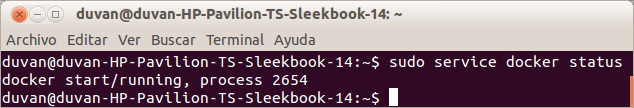
\includegraphics[scale=0.4]{1}   
			\caption{Correcta instalación del servicio Docker } 
		\end{figure}
		
	\item Descargar la imagen oficial de Docker para el software Apache Solr (Motor de búsqueda de código abierto)
		\begin{center}
			\texttt{sudo docker pull solr}
		\end{center}
	
			\begin{figure}[ht]
				\centering
				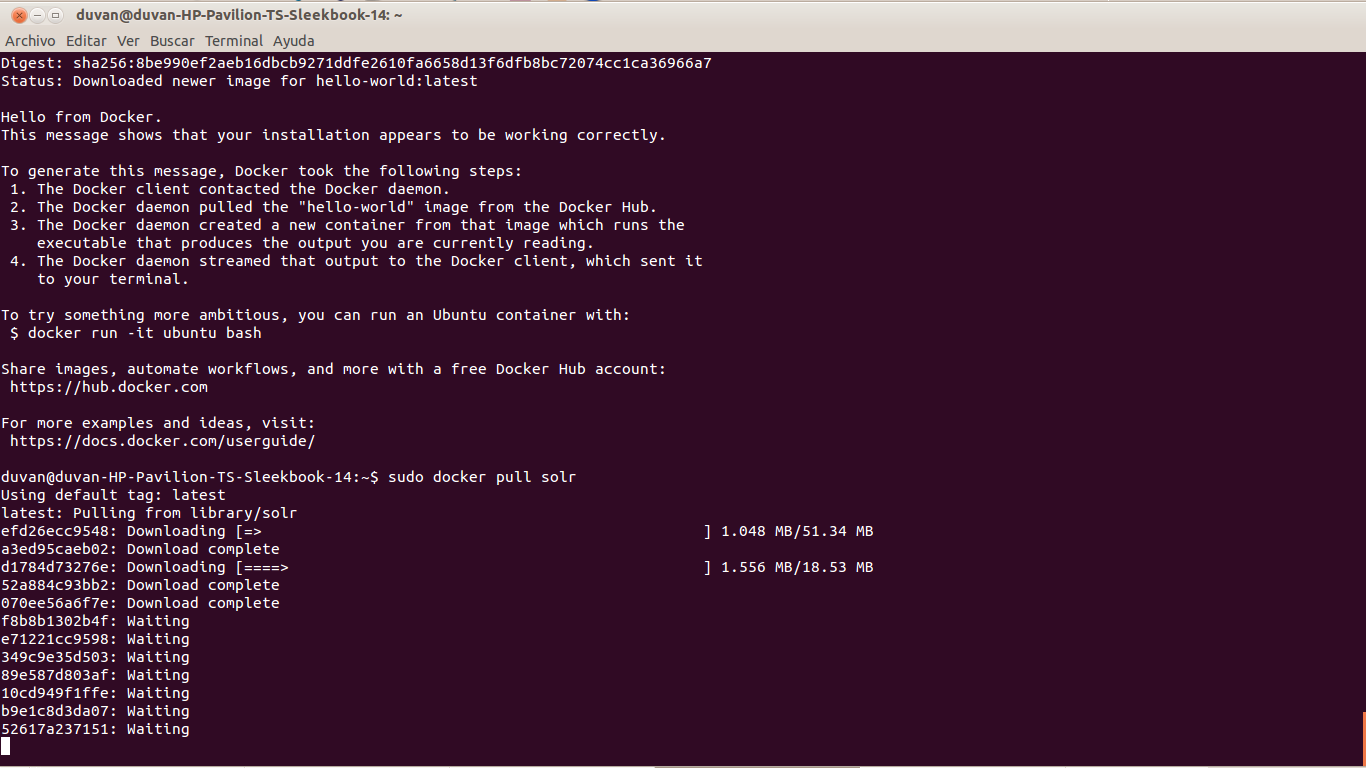
\includegraphics[scale=0.3]{2}   
				\caption{Descarga imagen Docker} 
			\end{figure}
	
		
	\item Listar las imágenes de Docker disponibles. Debe aparecer la imagen de \texttt{solr} descargada.\\
	
	
			\begin{center}
				\texttt{sudo docker images}
			\end{center}

			\begin{figure}[ht]
				\centering
				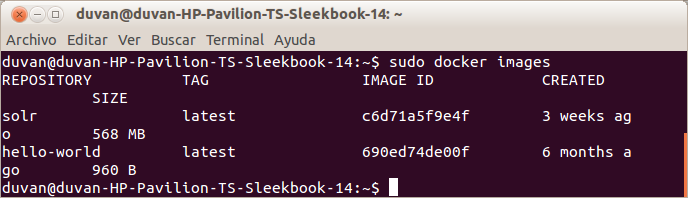
\includegraphics[scale=0.4]{3}   
				\caption{Listar las imágenes de Docker} 
			\end{figure}
	
	\item Iniciar el servidor de Apache Solr ejecutando un contenedor de Docker.
	
				\begin{center}
					\texttt{sudo docker run -p 8983:8983 -d -- name mysolr solr}
				\end{center}
				
			 		
				
	Este comando merece una explicación:\\
	
	\begin{itemize}
		\item \texttt{docker run} es el comando para ejecutar un nuevo contenedor Docker.\\
		 Este comando recibe varios parámetros.
		 \item \texttt{-p} especifica un mapeo de puertos, \texttt{<puerto-host>:<puerto-contenedor>} en donde se le dice que un puerto determinado en el huésped redirecciona al puerto del contenedor, usualmente el puerto de un servicio determinado. En este caso, 8983 es el puerto del servicio Solr.
		 \item \texttt{-d} especifica que el contenedor se va a ejecutar en \texttt{background}.
		 \item \texttt{--name} especifica un nombre para el contenedor. En el comando anterior, el contenedor se llama \texttt{mysolr}.
		 \item Cuando se lanza el contenedor, debe especificarse su imagen base; en este caso, \texttt{solr} es el nombre de la imagen.
	\end{itemize}
	
\begin{figure}[ht]
	\centering
	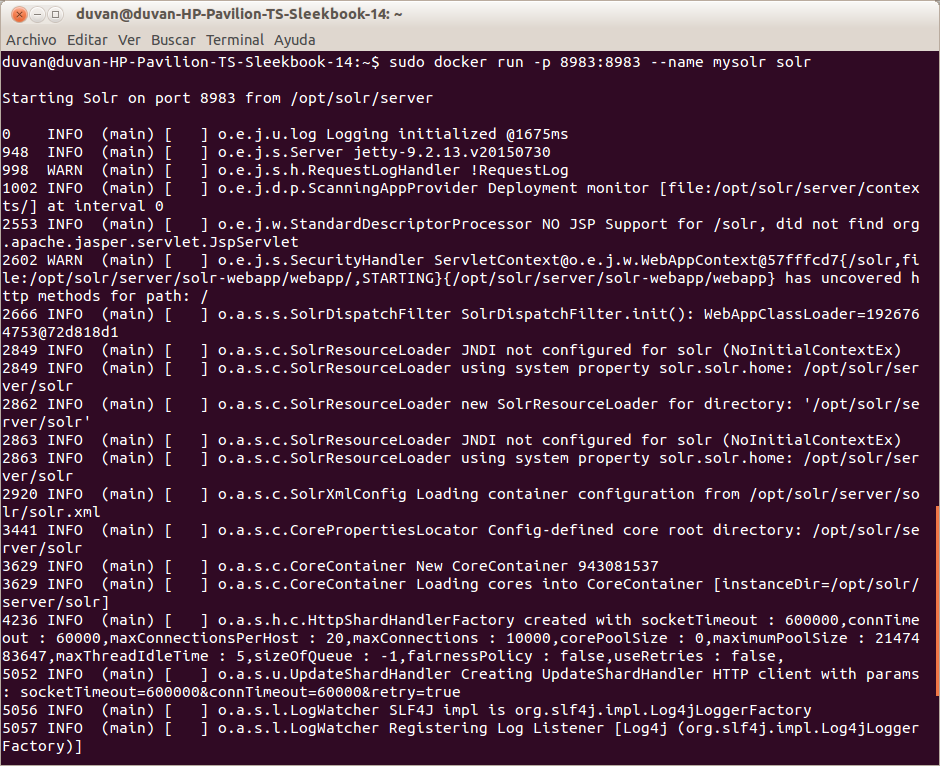
\includegraphics[scale=0.24]{4}   
	\caption{Iniciar el servidor de Apache Solr} 
\end{figure}	
	
\newpage
	\item Verificar que el contenedor se esté ejecutando. Para ello, ejecutar el comando
		\begin{center}
			\texttt{sudo docker ps}
		\end{center}
\begin{figure}[ht]
	\centering
	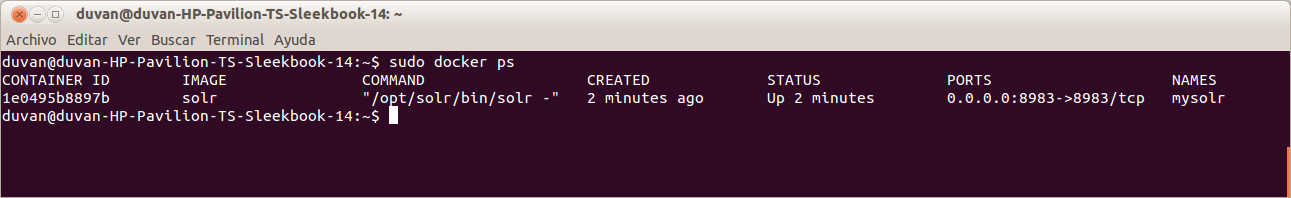
\includegraphics[scale=0.3]{5}   
	\caption{ Verificación que el contenedor se esté ejecutando} 
\end{figure}		
		
		
		\item En el anterior comando, se listan varias características del contenedor, incluido su identificador. Con este identificador, es posible acceder a los logs del contenedor, si es necesario verificar en detalle las acciones sobre el mismo.
		\begin{center}
			\texttt{sudo docker logs -f <id-contenedor>}
		\end{center}
\begin{figure}[ht]
	\centering
	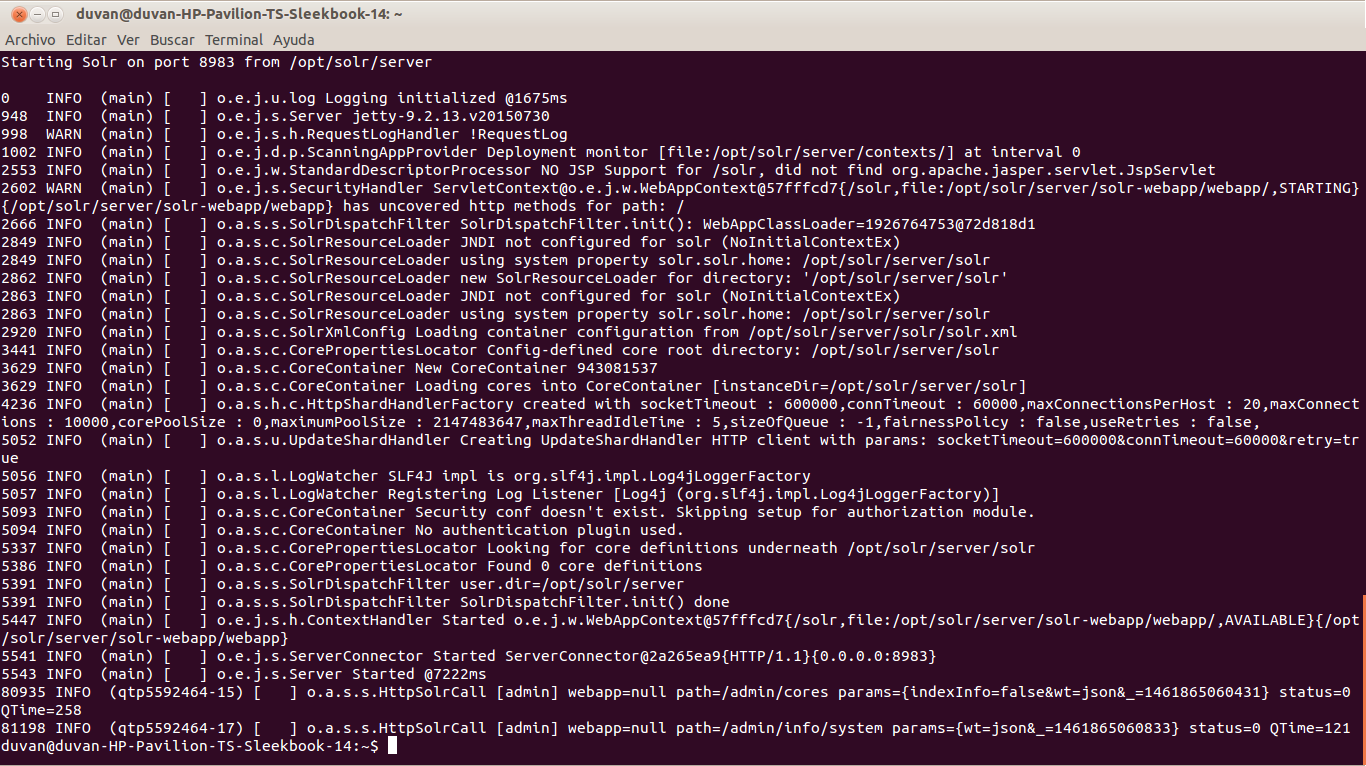
\includegraphics[scale=0.3]{6}   
	\caption{Logs del contenedor} 
\end{figure}	
\newpage		
		\item Acceder a la consola de administración del servidor Apache Solr. Para ello, desde un navegador ingresar a la URL  \href{http://127.0.0.1:89983}{\texttt{http://<direccion-huesped- docke>:89983}}
		
\begin{figure}[ht]
	\centering
	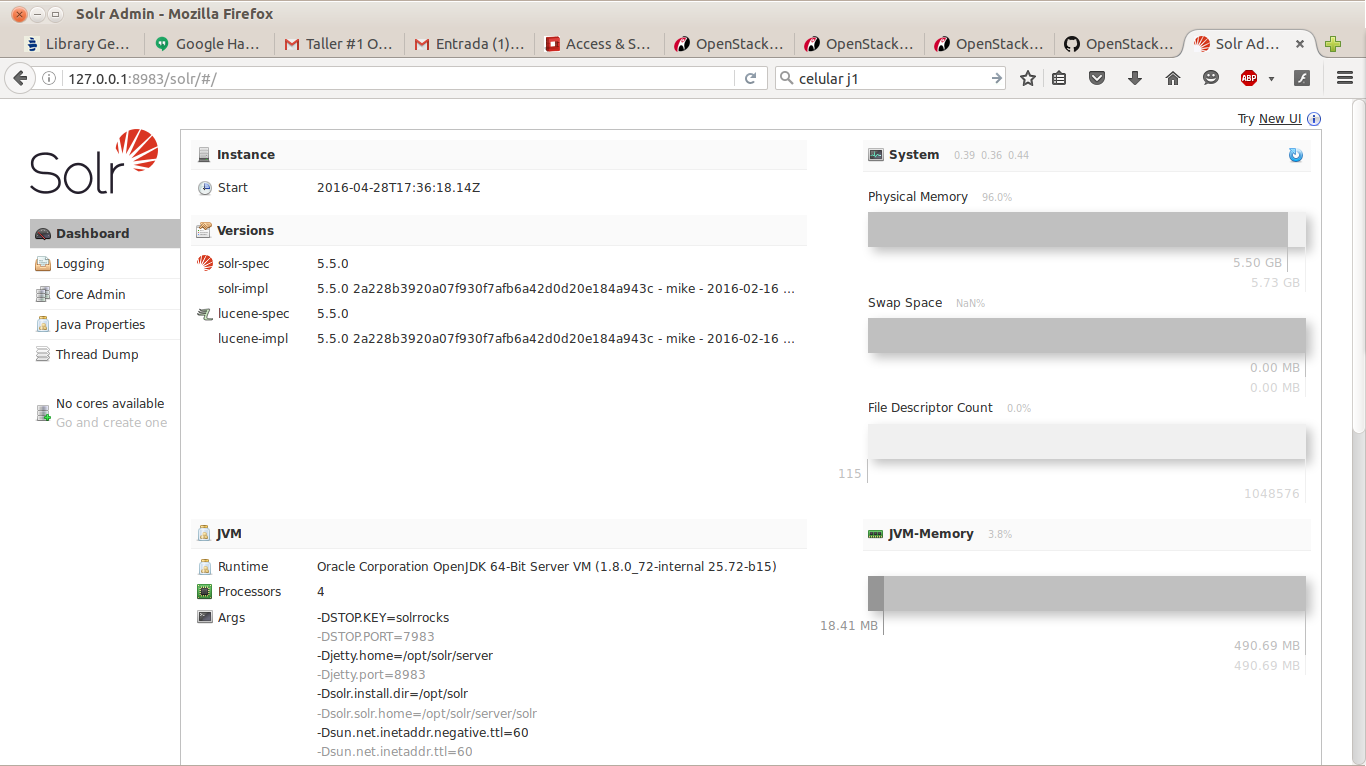
\includegraphics[scale=0.3]{7}   
	\caption{Logs del contenedor} 
\end{figure}
		
	\item 	En este momento, la aplicación ya está desplegada en el contenedor, disponible para utilización.  Por ejemplo, se desea utilizar el servidor Solr recién desplegado para crear un índice núcleo.  Lo primero es acceder a la consola del contenedor, ya que este se encuentra ejecutándose como un proceso en \textit{background}. 
	\begin{center}
		\texttt{sudo docker exec -it --user=solr mysolr bash}
	\end{center}
	\begin{figure}[ht]
		\centering
		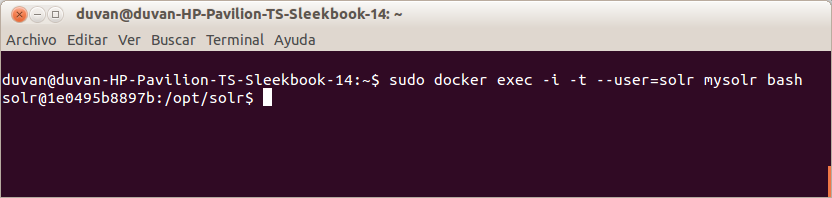
\includegraphics[scale=0.5]{8}   
		\caption{creación un índice núcleo} 
	\end{figure}		
	
	\newpage
	
	
	\item Ejecutar el comando
	\begin{center}
		\texttt{bin/solr create\_core -c gettingstarted}
	\end{center}
	\begin{figure}[H]
		\centering
		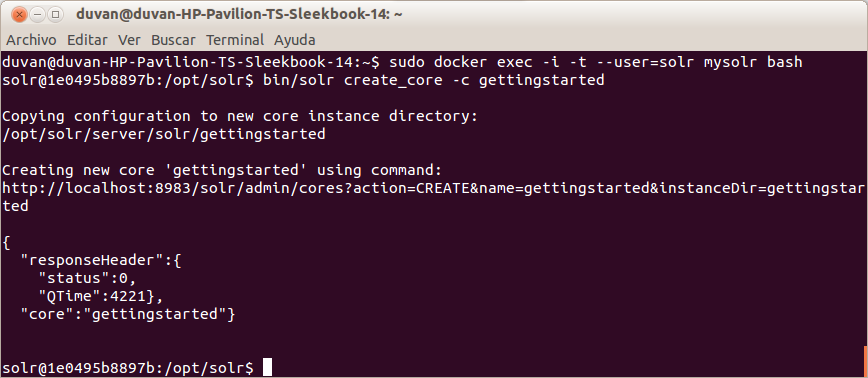
\includegraphics[scale=0.4]{9}   
		\caption{Resultado comando \texttt{bin/solr create\_core -c gettingstarted}} 
	\end{figure}


%%

\newpage	
	\item 	 Una de las funcionalidades más interesantes de Docker es poder copiar directamente un archivo creado en la máquina huésped a cualquier directorio dentro del contenedor. Para ello, crear en la máquina huésped (no en el contenedor) un archivo \texttt{\href{https://github.com/wilrilo/talleres/blob/master/file/taller6/solr.xml}{solr.xml}} con el siguiente contenido a manera de ejemplo:
	
	
	
\begin{small}
\begin{lstlisting}[frame=single]	
<add>
	<doc>
		<field name="id">SOLR1000</field>
		<field name="name">Solr, the Enterprise Search Server</field>
		<field name="manu">Apache Software Foundation</field>
		<field name="cat">software</field>
		<field name="cat">search</field>
		<field name="features">Advanced Full-Text Search Capabilities
		 using Lucene</field>
		<field name="features">Optimized for High Volume Web
		 Traffic</field>
		<field name="features">Standards Based Open Interfaces - XML
		 and HTTP</field>
		<field name="features">Comprehensive HTML Administration
		 Interfaces</field>
		<field name="features">Scalability - Efficient Replication to
		 other Solr Search Servers</field>
		<field name="features">Flexible and Adaptable with XML
		 configuration and Schema</field>
		<field name="features">Good unicode support: h&#xE9;llo (hello
		 with an accent over the e)</field>
		<field name="price">0</field>
		<field name="popularity">10</field>
		<field name="inStock">true</field>
		<field name="incubationdate_dt">2006-01-17T00:00:00.000Z</field>
	</doc>
</add>	
	\end{lstlisting}
\end{small}	
	

	\begin{figure}[ht]
		\centering
		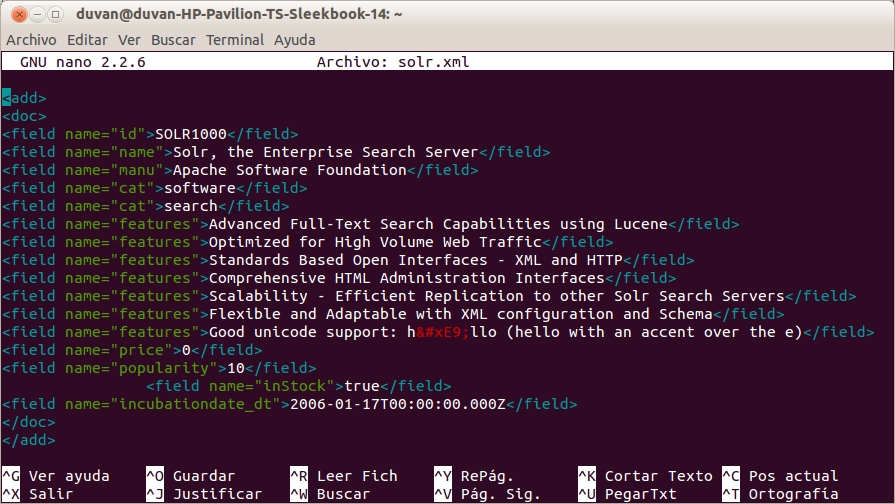
\includegraphics[scale=0.4]{10}   
		\caption{Modificación archivo \texttt{\href{https://github.com/wilrilo/talleres/blob/master/file/taller6/solr.xml}{solr.xml}}} 
	\end{figure}		

Acto seguido, copiar el archivo al directorio \texttt{/opt/solr} en el contenedor.  Reemplazar \texttt{<id-contenedor>} con el respectivo valor.	

\begin{center}
	\texttt{sudo docker cp solr.xml <id-contenedor>:/opt/solr/solr.xml}
\end{center}
\begin{figure}[ht]
	\centering
	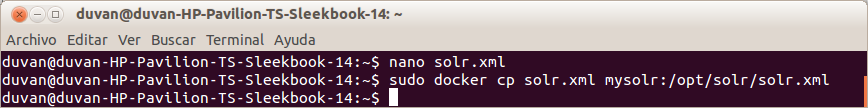
\includegraphics[scale=0.4]{101}   
	\caption{Copiado del archivo} 
\end{figure}
\newpage
\item Ingresar nuevamente a la consola. Verificar la existencia del archivo \texttt{solr.xml} y ejecutar el comando


\begin{center}
	\texttt{bin/post -c gettingstarted ./solr.xml}
\end{center}
\begin{figure}[ht]
	\centering
	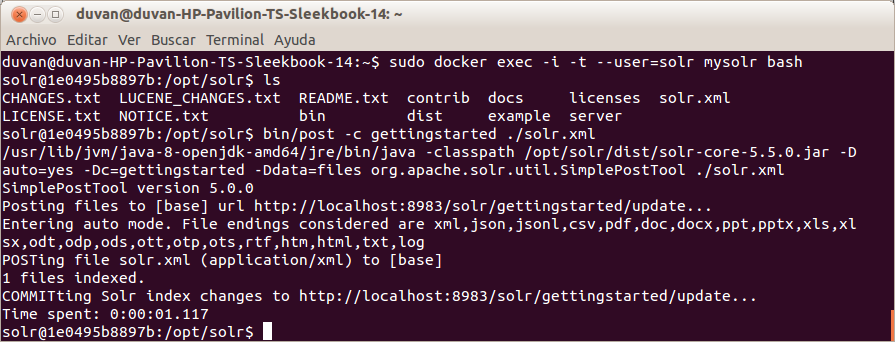
\includegraphics[scale=0.4]{11}   
	\caption{Verificación de la existencia del archivo \texttt{solr.xml}} 
\end{figure}

\item El anterior comando debe permitir indexar archivos en el servidor Solr. (El tutorial no trata directamente de Solr sino de Docker, luego no es necesario dominar completamente la consola de administración de Solr). Acceder a la consola de administración del Solr y verificar la indexación


\begin{figure}[H]
	\centering
	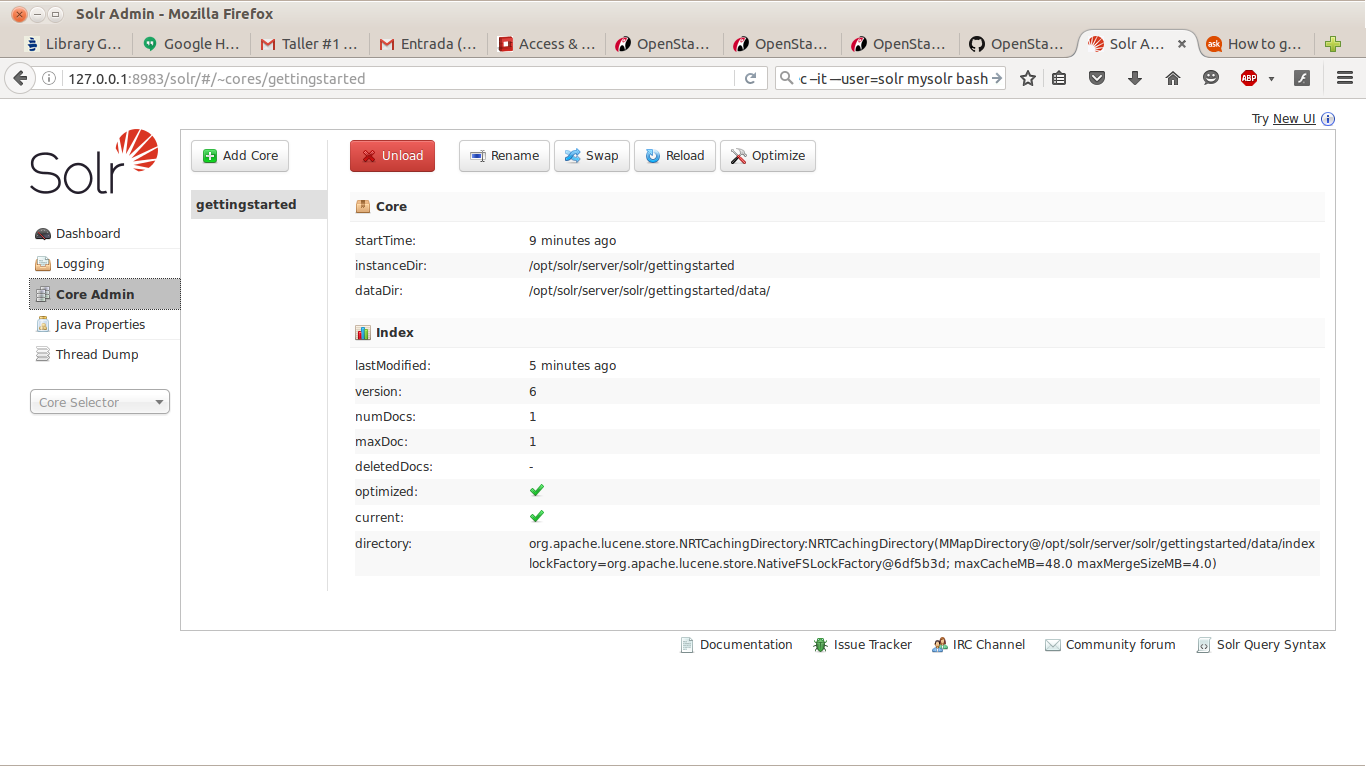
\includegraphics[scale=0.3]{12}   
	\caption{verificación de  la indexación} 
\end{figure}

\item Detener el contenedor

\begin{center}
	\texttt{sudo docker stop mysolr}
\end{center}

\begin{figure}[ht]
	\centering
	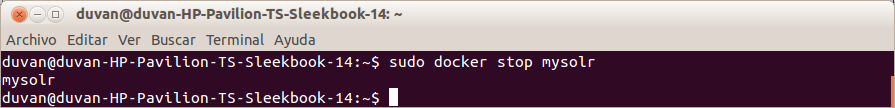
\includegraphics[scale=0.4]{13}   
	\caption{Comando para detener el contenedor} 
\end{figure}

Verificar que el contenedor aparezca como “\texttt{Exited}” en su estado después de ejecutar el comando  
\begin{center}
	\texttt{sudo docker ps -a}
\end{center}

\begin{figure}[ht]
	\centering
	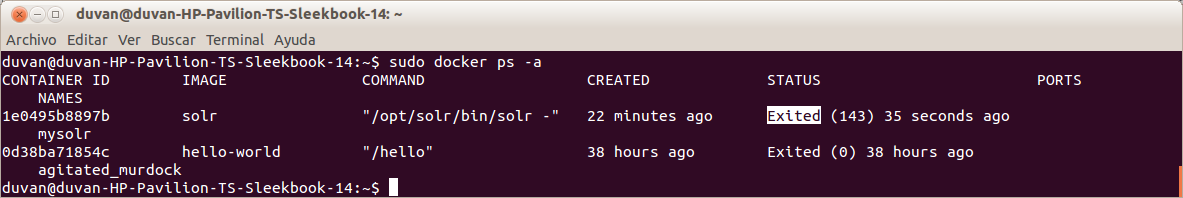
\includegraphics[scale=0.4]{131}   
	\caption{Verificación de la salida correcta del contenedor} 
\end{figure}


\item Eliminar el contenedor.  
\begin{center}
	\texttt{sudo docker rm mysolr}
\end{center}

\begin{figure}[H]
	\centering
	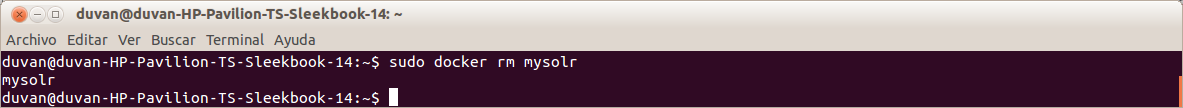
\includegraphics[scale=0.4]{14}   
	\caption{Eliminar contenedor} 
\end{figure}

\begin{figure}[ht]
	\centering
	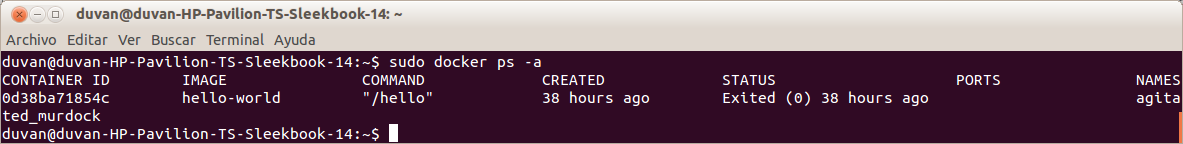
\includegraphics[scale=0.4]{141}   
	\caption{Contenedor eliminado} 
\end{figure}

\item En caso de requerirse, es posible eliminar la imagen utilizando el comando
%%

\begin{center}
	\texttt{sudo docker rmi solr}
\end{center}

\begin{figure}[H]
	\centering
	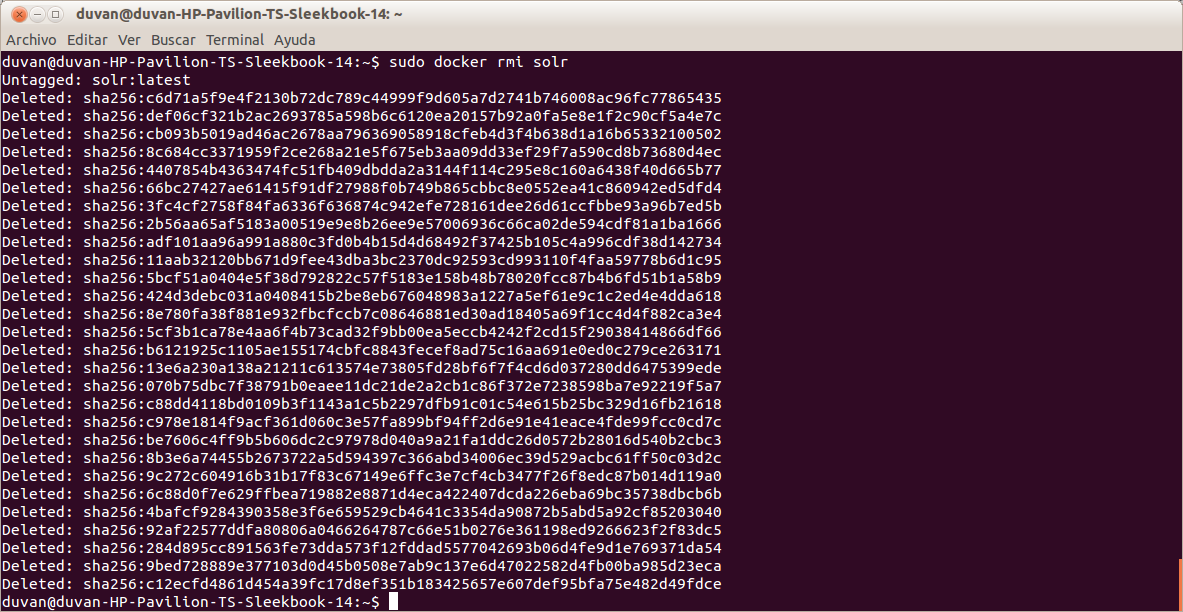
\includegraphics[scale=0.4]{15}   
	\caption{Eliminar la imagen} 
\end{figure}

\begin{figure}[ht]
	\centering
	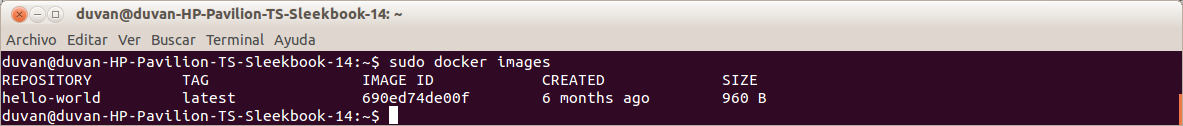
\includegraphics[scale=0.4]{151}   
	\caption{Imagen eliminado} 
\end{figure}

\end{enumerate}
\section{BIBLIOGRAFÍA}
	\begin{itemize}
		\item \href{https://www.docker.com/what-docker}{https://www.docker.com/what-docker}
	\end{itemize}
\end{document}
